%--- Jens:

\begin{frame}{SUSY theorie}
\begin{itemize}
\item symmetrie under spin transformation\\
\item MSSM has minimal new particles but over 100 free parameters\\
\item might solve GUT's and explains dark matter\\
\item quarks \& leptons $\rightarrow$ squarks \& sleptons (spin 0)\\
\item gauge bosons $\rightarrow$ gauginos (spin 1/2) 
\end{itemize}

\begin{figure}[B]
	\centering
	 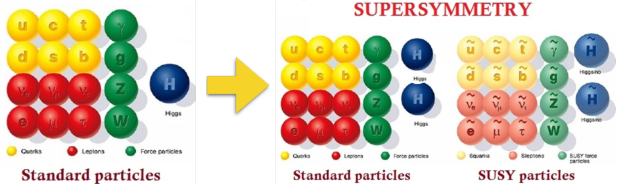
\includegraphics[width=1\textwidth,]{figures/mssm.png}
	\caption{Minimal supersymmetric standard model MSSM.
	 \begin{tiny}
	\qquad\qquad\qquad\qquad\qquad\qquad\qquad\qquad\qquad\qquad 
	source:  http://inspirehep.net/record/1407182/files/SUSY.png
	\end{tiny}}
\end{figure}

\end{frame}


\begin{frame}{LM6 \& LM9}

\begin{itemize}
\item concrete parameter setups leads to different branching ratios\\
\item LM6 \& LM9 have relative high cross sections\\ 
\item SUSY-processes: squark \& gluino pair production
\end{itemize}

\begin{figure}[H]
	\centering
	 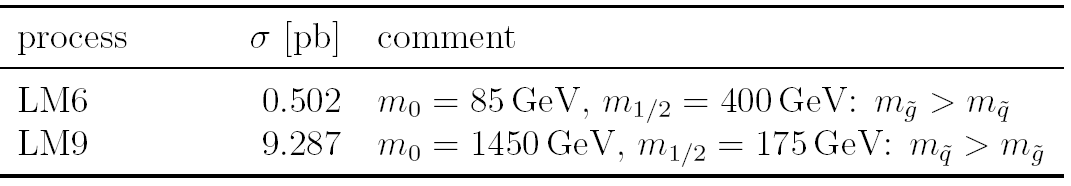
\includegraphics[width=\textwidth,]{figures/properties.png}
	%\caption{aus Übungsblatt Nr. 10}
\end{figure}

\end{frame}

\begin{frame}{SUSY im Detektor /Feynmangraphen, bkg-Prozesse  }

\begin{itemize}
\item quantum number $R=(-1)^{3B+L+2S} \quad R_{SM}=+1 \quad R_{SUSY}=-1$ \\
\item conservation of R-parity leads to stable ligthtest supersymmetric particles (LSP)\\
\item LSP is only weak interacting, detectable via $\slashed{H}_T$ \\
\item 2 susy processes: \quad $\tilde{g} \rightarrow \bar{q}+\tilde{q}$\\%;\quad  \tilde{q} \rightarrow q + LSP$; \quad leading to high $H_T$ and many jets\\
\item background: all processes with high $H_T, \slashed{H}_T$ and many jets:
$W(l\nu)+jets, Z(\nu\nu)+jets, t\bar{t}+jets, QCD$ 

\end{itemize}

\begin{figure}[H]
	\centering
	 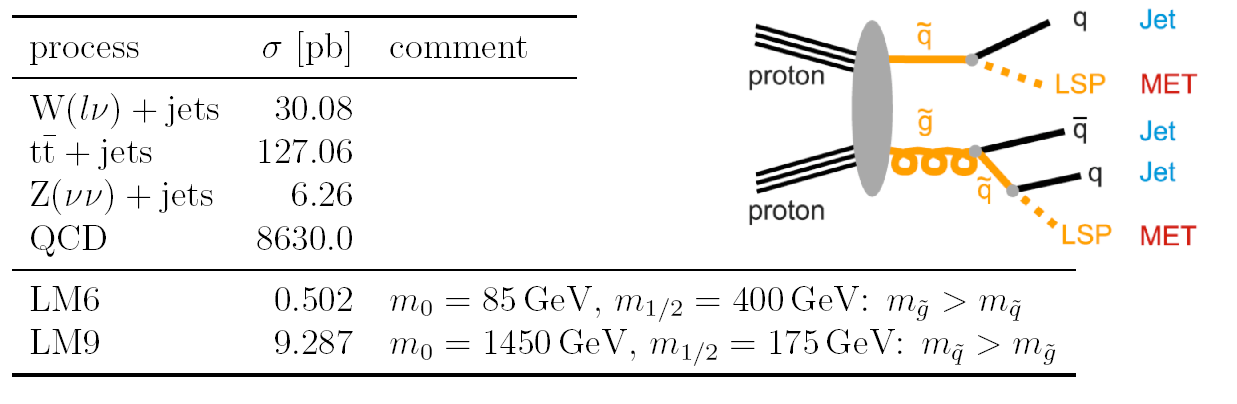
\includegraphics[width=0.8\textwidth,]{figures/feynman+bkg.png}
\end{figure}
\end{frame}



